\newlecture
\setcounter{chapter}{9}
\setcounter{section}{0}
\def\coursetopicnumber{I}
\def\textbookchapter{Course Topic I: Vectors and Vector-Valued Functions}
\def\topic{Functions of Several Variables and Three Dimensional Space} % this is the printed title
\def\shorttopic{Multivariable functions, 3D space} % short topic
\def\textbookname{Active Calculus} % this is the corresponding textbook
\def\shorttextbookname{AC} % this is the short name for the book
\def\textbooksection{9.1A} % corresponding textbook section
\def\textbooksectionurl{https://activecalculus.org/vector/S-9-1-Functions.html} % URL for textbook section
\def\handoutday{} % this is the printed date
\addtocontents{toc}{\large \textbookchapter \normalsize \medskip \par} %% for table of contents
%%%%%%%%% DOCUMENT CONTENT STARTS BELOW


\thispagestyle{plain}
\topstuff
\section{(9.1A) \topic{} \booklink{}}
In this section, we will learn about three dimensional space. We will do so in the context of functions of two variables. These notes correspond to the first half of the material in Section 9.1.

\subsection{Functions of several variables}
\begin{ex}
    Draw a circular cylinder with radius $r$ and height $h$. Find a formula for its volume.
\end{ex}

\vspace{1in}

The formula for the cylinder's volume $V$ depends on two variables: $r$ and $h$. Note that $r$ and $h$ don't necessarily have anything to do with each other. Thus, we call them \emph{independent variables}. Since $V$ depends on them, we call $V$ a \emph{function}, which we denote by 
\[
    V=\phantom{V(r,h).}\hspace{1in}
\]

\begin{ex}
    Come up with a combination of $r$ and $h$ for which the volume formula makes sense. Come up with a combination of $r$ and $h$ for which the volume formula doesn't make sense.
\end{ex}

\vspace{1.5in} 

\begin{ex}
    Evaluate $V(3,4)$. Explain what this calculation says.
\end{ex}

\vspace{1in}

\pagebreak 

\begin{defn}[Domain, Range]
    The \emph{domain} of a function is the set of inputs for which the function makes sense. The \emph{range} of a function is the set of outputs.
\end{defn}

\begin{ex}
    Describe the domain of the function $V(r,h)$ with a sentence.
\end{ex}

\vspace{1in}

\begin{ex}
    With the same function $V$ from before, draw the domain of the function $V(r,h)$.
\end{ex}

\vspace{1.3in}

\begin{ex}
    Is $V$ an increasing function of $r$, a decreasing function of $r$, or neither? How about with $h$?
\end{ex}

\vspace{.75in}

\begin{ex}
    Is 9 in the range of $V$?
\end{ex}

\vspace{.75in}

Here are two graphs of the function $V(r,h)=\pi r^2h$ for $0\le r\le 6$ and $0\le h\le 6$.
\begin{center}
    \iffalse
        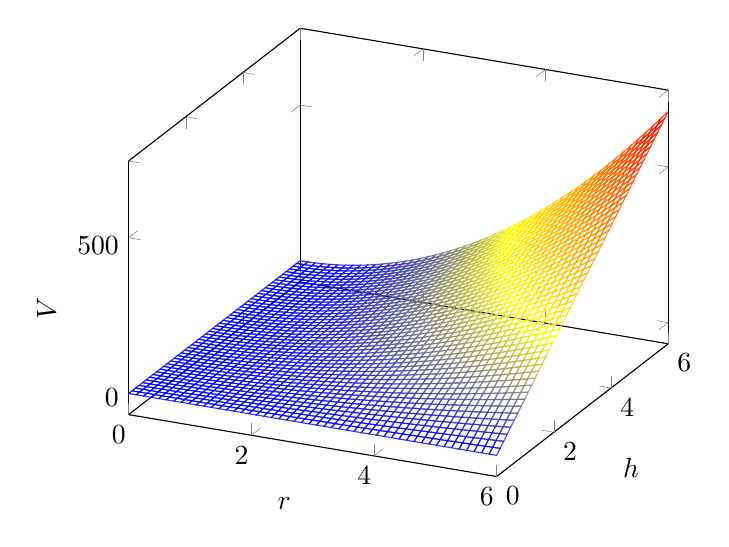
\begin{tikzpicture}
        \begin{axis}
        [xlabel={$r$}, ylabel={$h$}, zlabel={$V$}]
        \addplot3[
        surf,
        opacity=0.8,
        samples=50, samples y=50,
        domain=0:6, domain y=0:6, xlabel near ticks,
        mesh]
        {pi*x^2*y};
        \end{axis}
        \end{tikzpicture}
        %% picture now built in supplemental overleaf project to reduce compile time
    \fi
    \includegraphics[width=.4\textwidth]{tikz-pictures/section-9.1-pic1-first-3d-graph-v1.pdf}\hfill
    \includegraphics[width=.4\textwidth]{tikz-pictures/section-9.1-pic1-first-3d-graph-v2.pdf}\label{img:multivar-fn-graph}
\end{center}
You can produce a similar image at \url{https://wolframalpha.com} with the command 
\begin{center} 
    \href{https://www.wolframalpha.com/input/?i=plot+V%3Dpi*r%5E2*h+for+0%3C%3Dr%3C%3D6+and+0%3C%3Dh%3C%3D6}
    {\tt{plot V=pi*r\string^2*h for 0<=r<=6 and 0<=h<=6}}
\end{center}


\pagebreak 

Note that the domain of a function may depend on context (like the volume of a cylinder). If we are just given a mathematical function (with no context), then the domain consists of inputs for which the function is defined.

For our purposes, functions are most often undefined due to issues of:
\begin{itemize} 
    \item division by zero, 
    \item square root of a negative number, 
    \item logarithm of 0 or a negative number.
\end{itemize}

\begin{ex}
    Let $f(x,y)=4+5\sqrt{x^2+y}$. Sketch the domain of $f$.
\end{ex}

\vfill

\begin{ex}
    Let $g(x,y)=\dfrac{x+2y}{x^2-y^2}$. Sketch the domain of $g$.
\end{ex}

\vfill 

\pagebreak 

\subsection{Representing functions of two variables}
\begin{defn}[Graph of a function]
    The \emph{graph} of a function $f=f(x,y)$ is the set of points of the form $(x,y,f(x,y))$ where the point $(x,y)$ is in the domain of $f$.
\end{defn}
In other words, the graph of $f$ is the set of points $(x,y,z)$ where $z=f(x,y)$. The graph is called a \emph{surface}.

In any coordinate system, we need to make a choice about the directions of the axes. With three variables, we need three axes. This means 3D space!
\vspace{2in}

In order to represent 3D space visually, we use perspective drawing. We typically only draw the positive ends of each axis. In the drawing above, the $y$- and $z$-axes are essentially in the page, and the $x$-axis is coming out of the page at us.

Note how the axes are oriented with respect to each other! We use the ``right hand system.''%\footnote{Image below from \url{https://commons.wikimedia.org/wiki/File:Right_hand_rule_Cartesian_axes-permuted.svg}.} 

\begin{minipage}{.6\textwidth}
\begin{framed}
With your right hand, point your index finger in the direction of the positive $x$-axis and your middle finger in the direction of the positive $y$-axis. Your thumb will then point in the direction of the positive $z$-axis.
\end{framed}
\end{minipage}
\hfill \begin{minipage}{.3\textwidth}
\includegraphics[width=\textwidth]{images/right hand rule axes.png}\label{img:right-hand-axes}
\end{minipage}

Some notation:
\begin{itemize}
    \item $\mathbb{R}$ is the set of real numbers, which we visualize with the real number line.
    \item $\mathbb{R}^2$ is the set of ordered pairs of real numbers $(x,y)$, which we visualize as the plane.
    \item $\mathbb{R}^3$ is the set of ordered triples of real numbers $(x,y,z)$, which we visualize as 3D space.
\end{itemize}

\vfill

In $\mathbb{R}^2$, there are four \emph{quadrants}: I, II, III, IV. In Quadrant I, $x,y\ge0$.
\medskip 

In $\mathbb{R}^3$, there are eight \emph{octants}. The \emph{first octant} is the region where $x,y,z\ge0$.
\bigskip 

Here's another way to think of the right hand system. If you are at the positive end of the $z$-axis and you look at the origin, you'll see the $x$- and $y$-axes oriented just as we normally orient them in 2D space.

\vspace{.5in}

\pagebreak 
Going further, if we have a function $f=f(x,y,z)$ of three variables, then its graph is the set of points $(x,y,z,f(x,y,z))$ where the point $(x,y,z)$ is in the domain of $f$. In other words, this is the set of points $(x,y,z,w)$ where $w=f(x,y,z)$. This graph is in $\mathbb{R}^4$ (i.e., in 4D!), which makes it pretty tricky to visualize. We can use similar ideas to think about $\mathbb{R}^n$ for any $n\ge1$.

\subsection{Some standard equations in three-space}
In $\mathbb{R}^3$, we have three coordinate planes: the $xy$-plane, the $xz$-plane, and the $yz$-plane. Each plane contains the axes in its name.
\begin{ex}
    Draw the three coordinate planes.
\end{ex}

\vspace{2in}

Note that when we graph a function $f(x,y)$, the domain of $f$ is part of (or all of) the $xy$-plane.

\begin{ex}
    Draw the (separate) graphs of the equations $y=0$, $z=2$, and $x=3$ in $\mathbb{R}^3$.
\end{ex}

\vspace{2.5in}

Recall: In $\mathbb{R}^2$, the distance between the points $P=(x_0,y_0)$ and $Q=(x_1,y_1)$ is 
\[
    \phantom{\sqrt{(x_1-x_0)^2+(y_1-y_0)^2}.}
\]

\vspace{1in}

\pagebreak 

In $\mathbb{R}^3$, we have a similar formula. 
\begin{framed}
    The distance between the points $P=(x_0,y_0,z_0)$ and $Q=(x_1,y_1,z_1)$ in $\mathbb{R}^3$ is
    \[
        \phantom{\sqrt{(x_1-x_0)^2+(y_1-y_0)^2+(z_1-z_0)^2}.}
    \]
\end{framed}

This comes from using the Pythagorean Theorem twice. See \href{https://activecalculus.org/vector/S-9-1-Functions.html#A-9-1-4}{Activity 9.1.5} in the textbook for details. (It's straightforward. In $\mathbb{R}^2$, we want the length of a diagonal of a rectangle. In $\mathbb{R}^3$, we want the length of a diagonal of a rectangular box.)

Any sphere can be described as the set of all points that are a fixed distance from a particular point. If we want a sphere of radius $r$ centered at $(x_0,y_0,z_0)$, then we want all points $(x,y,z)$ which are distance $r$ from $(x_0,y_0,z_0)$. In other words, we want
\[
    \phantom{\sqrt{(x-x_0)^2+(y-y_0)^2+(z-z_0)^2}=r.}
\]
We can square both sides to eliminate the square root and get the following:
\begin{framed}
    The equation of a sphere of radius $r$ centered at the point $(x_0,y_0,z_0)$ is
    \[
        \phantom{(x-x_0)^2+(y-y_0)^2+(z-z_0)^2=r^2.}
    \]
\end{framed}
\begin{ex}
    Write down the equation of a sphere of radius 3 centered at the point $(2,-4,0)$.
\end{ex}

\vspace{1in}

For the next problem, we will ``complete the square.'' The key idea is that 
\[
    x^2+ax=\left(x+\dfrac{a}{2}\right)^2-\left(\dfrac{a}{2}\right)^2.\]
    \emph{(For a refresher on completing the square, check out \href{https://tutorial.math.lamar.edu/classes/alg/SolveQuadraticEqnsII.aspx}{Paul's Notes}.)}
\begin{ex}
    The equation $x^2+y^2+z^2+6x-2y+10z=14$ defines a sphere. Where is it centered and what is its radius?
\end{ex}
\vfill

